\chapter{Deterministic Chaos vs. Stochastic Turbulence}
\label{c_chaos}

In this chapter, I tackle the difficult question regarding the level of determinism of the turbulence in LAPD. Through the previous chapters, I maintained the modern 
Ruelle and Takens~\cite{ruelle1971} viewpoint that the turbulence is governed by a set of deterministic differential equations. That allowed me to simulate the turbulence using a set of differential
equations with non-random coefficients. However, I also largely used statistical and structural theory to diagnose the turbulence, assuming as most do, that the large number of degrees of freedom
available to the turbulence prevents a simpler diagnosis.
In this chapter, I explore this assumption regarding the number of relevant degrees of freedom, which is equivalent to the question of whether the turbulence in LAPD is deterministic
(governed by a few degrees of freedom) or stochastic (governed by many).
I am motivated by the recent work on LAPD by Pace, Shi, Maggs, and Morales
~\cite{pace2008a,pace2008b,shi2009,maggs2011,maggs2012a,maggs2012b,maggs2013}, which I review below. Their conjecture is that the plasma turbulence in LAPD and a number of other devices is deterministic.

\section{Lorentzian Pulses as an Indicator of Deterministic Chaos}
\label{s_lorentzian_pulses}

In this section, I explain some of the work by Pace, Shi, Maggs, and Morales, in which they identified exponential frequency spectra and 
Lorentzian pulses in the time signals of experimental measurements, leading them to the turbulence as deterministic chaos.
I do this while applying their findings to my experimental and simulation data, which should not be too much different than some of the data they used, especially that of Pace~\cite{pace2008a,pace2008b}.

Since they based most of their analysis and findings on time signals of experimental data rather than spatially resolved simulation data, 
I restrict myself here to looking at density and $I_{sat}$ time signals, neglecting simulated spatial structures.
While comparing time signals point for point is futile in chaotic systems due to sensitivity to initial conditions,
chaotic systems can produce time signals with identifiable visual characteristics.
In this regard, Pace et al. discovered that the time signals in LAPD experiments and in the edge of some magnetic confinement devices
are made up of Lorentzian-shaped pulses~\cite{pace2008a,pace2008b}. A Lorentzian is simply a function of the form

\beq
\label{lorentz_eqn}
f(t) = A/\left[1 + (t - t_0)^2/\tau^2 \right]
\eeq
where $A$ is the pulse amplitude, $t_0$ is its center, and $\tau$ is the pulse width. The absolute value of the Fourier transform of a Lorentzian is simply a decaying exponential, so
the Lorentzian pulses in the time signals lead to frequency power spectra that have exponential shape, which show up as a straight line in a log-linear plot. In such a plot, the slope of the line
is proportional to the Lorentzian width $\tau$. Sometimes, however, the Lorentzian
pulses in the time signals have different widths, which cause different spectral slopes, leading to power spectra with non-exponential shape. 

To compare my time signals to those of Pace and others, I first plot the frequency spectra of the experiment,
the Periodic simulation, and the $n=0$ suppressed simulation in Fig.~\ref{lorentzians} a). I don't use any window functions since they can distort any structures in the time signals,
and I use only one radial location (30 cm) rather than doing a volume average. Clearly, the spectra are not exponential for either the experiment or the simulations. This doesn't rule out
Lorentzian pulses in the time signals, however, as long as the time signals have pulses of varying width. So next, I look at the time signals of the experiment and simulations. I show representative
signals for the experiment, Periodic simulation, and $n=0$ suppressed simulation in Figs.~\ref{lorentzians} b), c), and d), respectively. Notice that the experiment and Periodic simulation
appear to have qualitatively similar time signals, while the $n=0$ suppressed simulation has a much different, simpler looking signal. Furthermore, the experiment and Periodic simulation contain
a number of pulse-like features. I take a closer look at some of these pulses in Figs.~\ref{lorentzians} e) (experiment) and f) (Periodic simulation), trying to find times when the pulses
are relatively isolated. In Fig.~\ref{lorentzians} e), I fit one of these pulses to a Lorentzian function (the dashed line), 
proving that this pulse, does in fact have a Lorentzian shape. I confirm that a Lorentzian does provide a better fit than a Gaussian, which doesn't fit the pulse as well for as long of a time
range as the Lorentzian. Furthermore, Gaussian pulses create spectra that look very different from those in Fig.~\ref{lorentzians} a), supporting the claim that the pulses have Lorentzian
rather than Gaussian shape. Finally, in Fig.~\ref{lorentzians} f),
I look at a signal snipet from the Periodic simulation with two relatively isolated pulses, and I fit a sum of two Lorentzian functions to this. Clearly, the fit is excellent as
both of these pulses have Lorentzian shape, and importantly, they have different widths, explaining the non-exponential shape of the spectra. I don't show a fit to the $n=0$ suppressed simulation
signal, but I note that it is quite sinusoidal with seemingly two or so dominant low frequency waves, which is clear from the highly peaked, non-broadband frequency spectra.

Now the reason why Lorentzian pulses show up in the time signals was explained by Maggs and Morales~\cite{maggs2012a}. They showed that some chaotic nonlinear systems -- including the well-known
Lorenz system~\cite{lorenz1963} -- undergo a certain kind of bifurcation, which they called a Lorentzian bifurcation. That is, some systems undergo a bifurcation from a solution that settles
on a limit cycle attractor to a solution that settles on a chaotic strange attractor, in which one of the variables has a trajectory made of Lorentzian pulses.
In a plasma, that trajectory is associated with an ${\bf E \times B}$ flow, which advects the scalar density and temperature, imprinting the Lorentzian shape onto their time signals.
The fact that experimental signals are made up of Lorentzian pulses, they say, indicates that the systems are deterministic and not stochastic because the systems are close to the bifurcation point
between the limit cycle and the strange attractor.

To understand this last important point, note that in general, dynamical systems have some control parameter associated with them that determines their steady state behavior. For instance, 
nuetral fluid behavior is often determined by the Reynolds number. As the control parameter increases, the system undergoes a series of bifurcations in which each bifurcation increases the effective
phase space dimension of the attractor. A limit cycle is a two-dimensional attractor. Strange attractors often have fractional dimension greater than two~\cite{manneville2004}.
The bifurcation from a limit cycle attractor to strange attractor then increases the dimension, or equivalently increases the effective number of degrees of freedom available to the system.
As the bifurcation parameter increases still further, the number of effective degrees of freedom increases, eventually becoming high enough for the system to be more stochastic than deterministic.
Any system then, near the bifurcation point between limit cycle and strange attractors will have a small number of degrees of freedom, making it deterministic.

For LAPD and similar plasma systems, the control parameters ought to be proportional to the equilibrium gradients. 
For the system to display Lorentzian chaotic dynamics, the conjecture is that the control parameter and thus the gradient must be high enough so that the attractor is not
a limit cycle, but low enough so that it still has a Lorentzian trajectory associated with it.
Furthermore, such a situation may be a natural consequence of chaotic advection in confinement-like systems because chaos causes
transport which relaxes the gradients and prevents them from building up. The control parameter, thereforem should not be able to grow much beyond the point where chaos ensues. 
In other words, the control parameter
causes the chaos, but the chaos regulates the the control parameter, preventing the system from straying from the bifurcation point between the limit cycle and the low dimensional strange attractor.

I note, however, that this is less likely to be the case in LAPD than in confinement devices like tokamaks. The reason is that LAPD sustains particle losses primarily through parallel transport
to the ends of the machine rather than through radial transport. That is, the radial confinement time is greater than the parallel confinement time in LAPD, which is different than the situation
in all but the SOLs of confinement devices. Therefore, the chaotic or turbulent advection does not have a chance to completely relax the profiles to the point where this advection is shut off.
That means that LAPD should be able to sustain a control parameter well above the chaotic threshold, allowing for high dimensional chaos, which is stochastic turbulence. I attempt to determine whether
the chaos is low or high dimensional in the following sections.

\begin{figure}[!]
\centerline{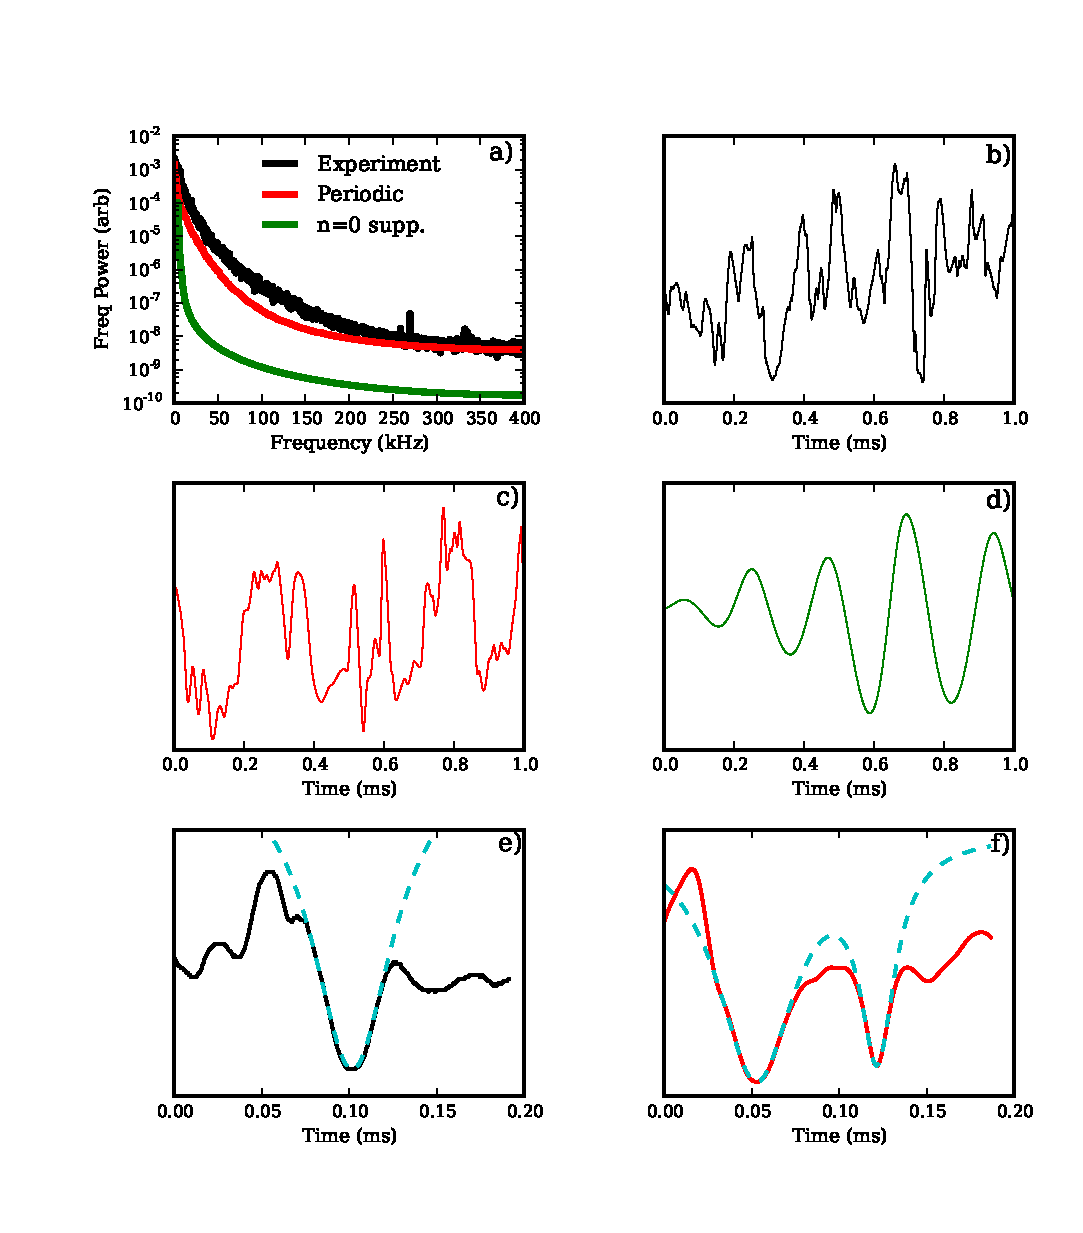
\includegraphics[]{lorentzians}}
\caption{Lorentzian pulses in time signals}
\label{lorentzians}
\end{figure}


\section{Permutation entropy as an Indicator of Chaos}
\label{s_ent_comp}

While Lorentzian pulses in the time signals of experimental data provided the clue to the possible chaotic nature of the turbulence in LAPD, there are more direct and more conclusive ways
to determine how deterministic versus how stochastic a system is. Therefore, Maggs and Morales set out to test one of their LAPD experiments with one of these more direct methods~\cite{maggs2013},
namely a method invented by Bandt and Pompe about a decade ago~\cite{bandt2002}. The Bandt-Pompe method, called permutation entropy, uses a
time signal of a single observable to quantify the amount of determinism of the underlying process that creates the time signal. The method has gained better theoretical
interpretation over the years, and various researchers have refined its implementation. Recently, Riedl et al.~\cite{riedle2013} published a review on permutation entropy that provides theory,
instructions, and most importantly, practical considerations for using the Bandt-Pompe method. In light of this review based on dozens of researchers' experience, I follow the procedures and lessons
in it rather than those in the Maggs and Morales paper.

\subsection{Trajectory reconstruction by the method of delays}
\label{ss_delays}

The Bandt-Pompe permutation entropy is partly based on a standard chaotic time signal analysis technique that is often called the method of delays, 
first formalized by Takens~\cite{takens1981}. The method of delays attempts to reconstruct the trajectory of an attractor on a manifold in the phase space over which the effective dynamics
take place. I review the method following Manneville's treatment~\cite{manneville2004}, but I note that there is another nice review that is more freely available by Theiler~\cite{theiler1990}.

First, one can formally write the dynamical system $\mathbf{\dot{X}} = \mathbf{\mathcal{F}} (\mathbf{X})$ for the state $\mathbf{X}$ in the phase space $\mathbb{X}$. Furthermore,
there is a manifold $\mathbb{M}$ of dimension $d_{\rm{eff}}$ on which the dynamics lie, where  $d_{\rm{eff}}$ is less than the dimension of the entire space $\mathbb{X}$. The only available
information is the time signal $W$ that is measured in an experiment. 
It is some unknown projection of the state $\mathbf{X}$ onto a single dimension: $W = \mathcal{W} ({\mathbf{X}})$. 
For a discrete time signal, the dynamical system may be approximated as

\beq
\label{dyn_sys_approx}
{\mathbf{X}}_{k+1} = {\mathbf{\mathcal{F}}} ({\mathbf{X}}_k)
\eeq
where the subscript denotes a time index. Reconstructing the dynamics amounts to determining an empirical relation between the ${\mathbf{X}}_k$ in their phase space and the observables
$W_k, k=0,1, \ldots$ Clearly, $W_0 = {\mathcal{W}}({\mathbf{X}}_0)$ is not sufficient to determine ${\mathbf{X}}_0$ since one coordinate is not enough to define ${\mathbf{X}}_0$. But, note that
$W_1$ is to the projection of ${\mathbf{X}}_1$, which evolves from ${\mathbf{X}}_0$ under the map $\mathbf{\mathcal{F}}$. Thus, the second measurement $W_1$ adds a piece of information
about the coordinate ${\mathbf{X}}_0$ through $W_1 = {\mathcal{W}}({\mathbf{X}}_1) = {\mathcal{W}}({\mathcal{\mathbf{F}}} ({\mathbf{X}}_0))$. The third measurement, $W_2$ further provides information
on ${\mathbf{X}}_0$ through $W_2 = {\mathcal{W}}({\mathcal{F}} ({\mathcal{F}} ({\mathbf{X}}_0)))$. 
In principle, a sufficiently long array of measurements of length $d_{\rm{test}}$, $\{W_0, W_1, \ldots , W_{d_{\rm{test}}-1}\}$ should serve to specify
${\mathbf{X}}_0$. Similarly, $\{W_1, \ldots , W_{d_{\rm{test}}}\}$ specifies ${\mathbf{X}}_1$, etc. 
Eventually, a whole trajectory ${\mathbf{X}}_k, k=0,1,\ldots$ can be reconstructed from the series of vectors,
${\mathbf{V}}_k = \{W_k, \ldots , W_{k+d_{\rm{test}}-1}\}$, existing in ${\mathbb{R}}^{d_{\rm{test}}}$.

The length $d_{\rm{test}}$ of the reconstruction vectors can be increased until the method produces a reliable reconstruction of the trajectory. $d_{\rm{test}}$ must be large enough so that one does
not lose any useful dynamical information. This means that different states must also have different reconstructions:

\beq
\label{diff_recons}
{\mathbf{X}}_k \ne {\mathbf{X}}_{k'} \rightarrow {\mathbf{V}}_k \ne {\mathbf{V}}_{k'}
\eeq

The tentative number $d_{\rm{test}}$ of components used to reconstruct the state vectors is more properly regarded as the effective dimension of the space in which the effective phase space
can be imbedded by means of an injective map. Thus, I change notation from $d_{\rm{test}}$ to $d_e$, the embedding dimension. Takens theorem states that the ${\mathbf{V}}_k$ achieve
a reliable reconstruction provided that the $d_e$ are large enough: $d_e \ge 2 d_{\rm{eff}} + 1$. In chaotic systems, strange attractors often have fractal dimension, $d_f$, and one can
replace $d_{\rm{eff}}$ by $d_f$ in this inequality.

Moreover, the ${\mathbf{V}}_k$ can actually be any series of $d_e$ measurements, namely, ${\mathbf{V}}_k = [W_k, W_{k + \kappa_1}, \ldots, W_{k + \kappa_{d_e-1}}]$, where the $\kappa_q$ can take on
any values. It's natural to take the $\kappa_q$ as multiples of some basic $\kappa$ so that ${\mathbf{V}}_k = [W_k, W_{k + \tau}, \ldots, W_{k + (d_e-1)\tau}]$, where $\tau$ is the subsampling
rate.

In practice, the usefulness of the method of delays relies upon choosing optimal values for the two basic ingredients in the reconstruction: 
the embedding dimension $d_e$ and the subsampling rate $\tau$ ($\tau$ is really a time, not a rate). 
Optimal values can reduce the effects of noise on results and can minimize required computation and required length of time signals.
The generally accepted optimal choice for the subsampling rate $\tau$ is the time over which a signal becomes decorrelated with itself~\cite{manneville2004,riedle2013}.
While the autocorrelation time seems like a natural quantity to use, it doesn't always lead to a satisfactory choice of $\tau$. A better criterion resting on solid theoretical arguments
revoles around the use of a quantity called the mutual information, which is defined as

\beq
\label{mutual_info}
I_{mut}(\tau) = \sum_{W',W''} P_{\tau}(W',W'') \rm{ln} \left( \frac{P_{\tau}(W',W'')}{P(W') P(W'')}  \right)
\eeq
where $W' = W_k, W'' = W_{k+\tau}$, $P(W)$ is the probability distribution of the time signal $W$, and $P(W',W'')$ is the joint probability distribution function of the signals $W'$ and $W''$.
$I_{mut}(\tau)$ is a measure of the redundance in the signal. When $\tau$ is small, the signals $W'$ and $W''$ are highly correlated and $I_{mut}$ is large, but when $\tau$ is large and the
signals are uncorrelated, $P_{\tau}(W',W'')$ is essentially $P(W') P(W'')$, making $I_{mut}$ small.

\begin{figure}[!ht]
\centerline{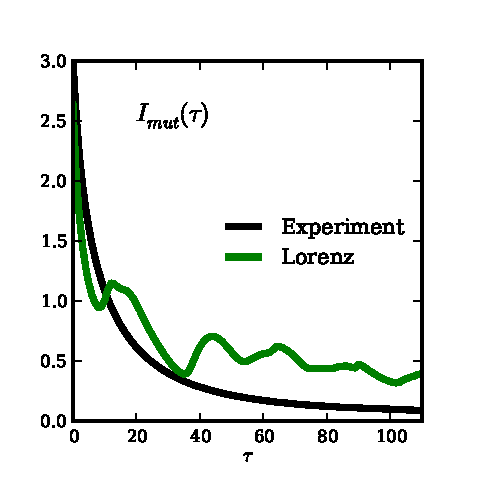
\includegraphics[]{imut}}
\caption{Mutual information as a function of subsampling rate}
\label{imut}
\end{figure}

In Fig.~\ref{imut}, I show an example of $I_{mut}(\tau)$ for two time signals. The black curve is the mutual information of the experimental $I_{sat}$ time signal at one radial location.
The green curve is the mutual information of the $x$ coordinate of the Lorenz model~\cite{lorenz1963}:

\beq
\label{lorenz_model}
\dot{x} = \sigma(y-x)   \qquad \dot{y} =  x(\rho-z) - y  \qquad \dot{z} = xy - \beta z
\eeq
where I use the well-know chaos-producing values $\sigma=10, \rho=28,$ and $\beta = 8/3$. I numerically solve the Lorenz model with an integration time step $0.017$ using a Python ODE solver.
The Lorenz model has an oscillating and decaying $I_{mut}(\tau)$, while the experiment has a simple decaying mutual information. The optimal value of $\tau$ corresponds to the first local minimum
of $I_{mut}$, which for the Lorenz model is at $\tau \approx 10$. The experiment has no local minimum, which can mean that there is either very large noise, the observable has been undersampled,
or that too many degrees of freedom are involved~\cite{manneville2004}. All of these can be a problem for using methods of low dimensional deterministic dynamical systems. However, in the next
section I review the permutation entropy, which can provide an optimal $\tau$ for the experiment. Furthermore, the permutation entropy can provide an optimal value for the embedding dimension
$d_e$. There are other methods for finding the optimal $d_e$, such as the method of false neighbors~\cite{manneville2004}, but I don't use it because it is difficult to analyze.

\subsection{Permutation Entropy}
\label{ss_pe}

\begin{figure}[!ht]
\centerline{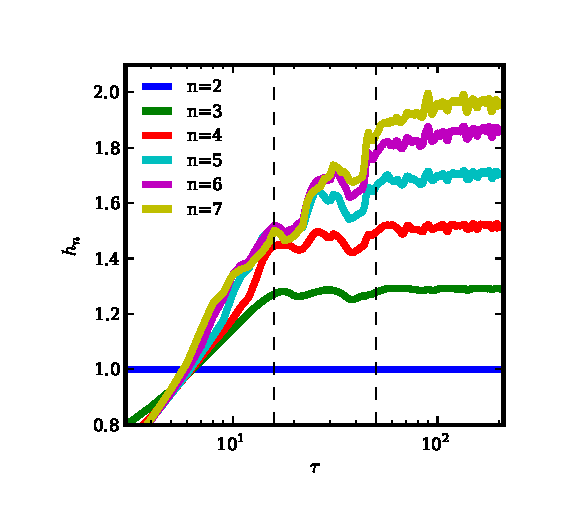
\includegraphics[]{pe_lorenz}}
\caption{Permutation entropy for the Lorenz model}
\label{pe_lorenz}
\end{figure}

The permutation entropy invented by Bandt and Pompe~\cite{bandt2002} defines a measure of the entropy of the time delay phase reconstructions based on their ordinal ranks. Specifically,
the time delay embedding vectors ${\mathbf{V}}_k$ with embedding dimension $d_e = n$ are binned into $n!$ bins based on the order of their elements. For instance, if $n=3$ and there is a vector,
${\mathbf{V}}_0 = (10,15,8)$, one counts this vector as one that has an rank representation of $(2,3,1)$. There are $3!=6$ different possible permutations of the ranked vectors. 
The number of vectors of a given ranked representation divided by the total number of embedding vectors produces a series of probabilities $p_j$ that add up to 1. The Shannon permutation entropy
is then defined by

\beq
\label{perm_ent}
P_n = - \sum_{j=1}^{n!} p_j {\rm{log}}_2 (p_j)
\eeq
It is also convenient to define different normalizations for the permutation entropy, such as $h_n = P_n/(n-1)$, which allows for entropies with different $n$ to be compared, and
$H_n = P_n/{\rm{log}}_2 (N)$, which ranges from $0 \le H_n \le 1$. More details on the procedure for calculating the permutation entropy may be found in Riedle et al.~\cite{riedle2013}.

The procedure of ranking the components of the time delay reconstruction vectors removes information regarding the phase space trajectory of the system.
The ranking procedure partitians or bins the phase space, erasing detailed information of the location of the trajectory. Nevertheless, the ranked vector counting provides a good measure of how
often a trajectory visits one of the phase space bins, revealing information regarding the stochasticity of the attractor. In general, the permutation entropy highlights underlying features
of attractor trajectories that are well-known from various other analyses. Furthermore, it is generally much easier to use than other methods.

Since the permutation entropy relies on time delay reconstructions of phase space trajectories, it is important to use properly reconstructed vectors in the analysis. That means, one must use
optimal values of the subsampling rate $\tau$ and the embedding dimension $n$ for the permutation entropy to have any meaning. The strong dependence of the permutation entropy on these
parameters makes it meaningless to compare the permutation entropy across different systems if the wrong parameters are used. 
I illustrate this strong dependence by calculating the permutation entropy for the Lorenz model
with varying values of $\tau$ and $n$, shown in Fig.~\ref{pe_lorenz}. For the different curves, I use different embedding dimensions $n$. The horizontal axis is a function of the subsampling rate
$\tau$. I divide the space into three separate regions, which I separate with the vertical dashed lines. The first region, from $1 \le \tau \le 16$ is the region where the permutation rises
monotonically with $\tau$. This rise is due to the under-subsampling in the reconstructed vectors, which is sometimes called the ``redundancy effect''~\cite{riedle2013}. The components in the
reconstructed vectors are too highly correlated, which causes the reconstructed trajectory to visit only limit regions of phase space. The reconstructed trajectories are poor representatives
of the original trajectories when the reconstructed vectors are under-subsampled. The region between the two dashed lines $16 \le \tau \le 50$ marks where 
the components of the reconstructed vectors become less correlated. 
For $\tau > 50$ components in the vectors are uncorrelated with their neighbor components, and the permutation entropy is relatively flat because the components cannot become any more decorrelated. 
This is called the ``irrelevance effect.''

Riedle et al. propose using the value of $\tau$ at the first dashed line, which in this case is $16$. Note that this is about double what I found for the optimal value based on the mutual information
analysis, but the different values produce permutation entropies that differ by only about $15\%$, so they do somewhat agree. Furthermore, other chaotic models that I have tested agree better.
As for the embedding dimension, they recommend using the value of $n$ that produces the highest permutation entropy at the location of the first dashed line. For the Lorenz model, this is
$n=6$, although $n=5$ has a permutation entropy that is nearly as large at the optimal value of $\tau$. The embedding dimension, as required by Takens theorem~\cite{takens1981}, which I discussed
above, must be $d_e \ge 2 d_f + 1$. Since the fractal dimension $d_f$ of the Lorenz model is known to be $2.06$, it requires an embedding dimension of $6$, just what the permutation entropy
analysis suggests. And an embedding dimension of $5$ would not do too poorly either.

A final point regarding the calculation of the permutation entropy deals with the total number of time points that are needed to calculate it. The probability distributions that go into
Eq.~\ref{perm_ent} of course become steadier as more reconstructed vectors are used, so the more time points the better. Actually, the number of vectors is more important than the number
of time points, and since the number of vectors decreases with increasing $\tau$, it is the total time used that's important. In general, Riedle et al. recommend using at least $5 n!$
vectors, which puts practical limits on the embedding dimension since $n!$ grows so fast with $n$. One may consider reconstructing extra vectors by changing the starting location of
the reconstructions. For instance, reconstructing vectors with time indices $[0,10,20,30,40]$, $[1,11,21,31,41]$, etc., where $\tau=10$, can give more reconstructed vectors than if one
throws out the vectors $[1,11,21,31,41] \ldots [9,19,29,39,49]$. However, there is little new information from vectors $[1,11,21,31,41] \ldots [9,19,29,39,49]$ because they are
highly correlated to vector $[0,10,20,30,40]$. So this doesn't significantly help. The permutation entropy is then quite limited to systems with small attractor
dimensions. The same is true for other techniques of low-dimensional deterministic chaos.

\begin{figure}[!ht]
\centerline{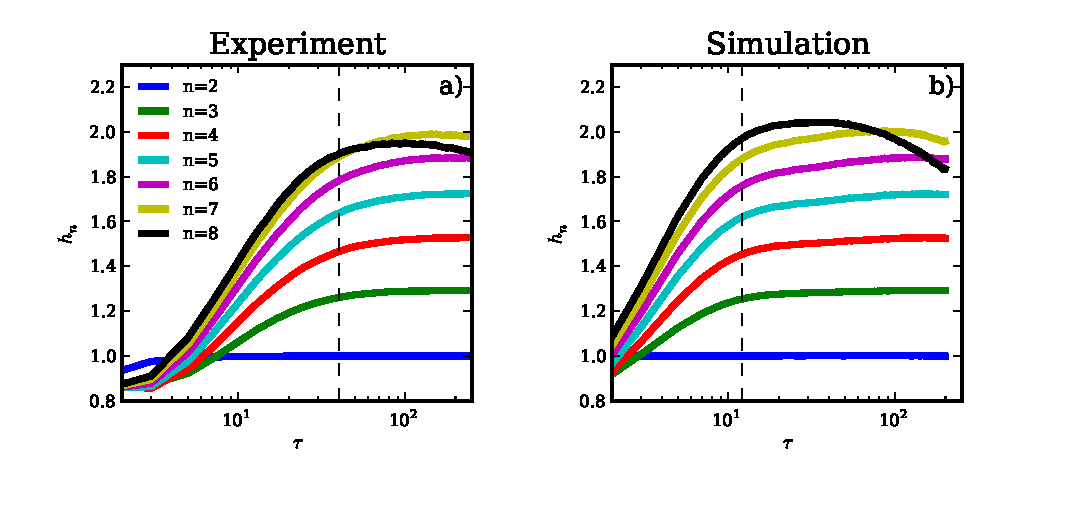
\includegraphics[]{pe_lapd}}
\caption{Permutation entropy for the experiment and simulation}
\label{pe_lapd}
\end{figure}

Moving on, I do the same permutation entropy analysis for the LAPD experiment and the Periodic simulation, which I show in Fig.~\ref{pe_lapd}. Like the Lorenz model, these curves all go
through a period of the redundancy effect and eventually reach a point at which the irrelevance effect sets in. The region between these two effects is harder to see, but that is not important.
One important effect, however, is the falloff of the entropy for high $\tau$ and high $n$. This is a result of using too few reconstructing vectors (fewer for the experiment), 
and it places a practical limit on the analysis at $n \sim 8$ (not to mention the time it takes to calculate the entropy as $n$ becomes this large).
Moreover, the experiment and simulation have different optimal subsampling rates: $40$ and $12$, respectively, but this is not meaningful since the original sampling is not the same. Essentially, the
experiment and simulation have the same permutation entropy curves, further validating the simulation. 
They both have significantly higher permutation entropies than the Lorenz model: $h_{n,{\rm{lapd}}} > 2$ compared to $h_{n,{\rm{Lorenz}}} = 1.5$. However, it is clear that the
permutation entropy at the dashed line is still rising as $n$ increases, meaning that the optimal embedding dimension is above $8$. And I cannot increase the embedding dimension without significantly
increasing the time of the experiment and the simulation. The permutation entropy, therefore, cannot be accurately calculated for the turbulence in LAPD. The turbulence simply has too many effective
degrees of freedom.

Nevertheless, I continue with the permutation entropy analysis, focusing now on the complexity of the time signals in addition to the entropy. The Jenson-Shannon complexity is 
defined by~\cite{rosso2007}

\beq
\label{csj}
C_S^J = -2 \frac{P_n(\frac{p +p_e}{2}) - \frac{1}{2} P_n(p) - \frac{1}{2} P_n(p_e)}{\frac{N+1}{N} {\rm{log}}_2(N+1) - 2 {\rm{log}}_2(2 N) + {\rm{log}}_2(N)} H_n(p)
\eeq
where $P_n$ is the Shannon permutation entropy defined in Eq.~\ref{perm_ent}. $P_n(p)$ refers to the normal permutation entropy. $P_n(p_e)$ refers to the maximum entropy, which occurs for
$p_j = 1/N, j=1,2,\ldots,N$. $H_n$ stands for the permutation entropy normalized by ${\rm{log}}_2(N)$, which takes on values in the range of $0$ to $1$. The complexity provides an important
additional piece of information that the entropy alone does not, namely, it quantifies the correlational degree of structures. Most importantly, chaotic and stochastic processes occupy
different locations in the entropy-complexity (CH) plane, which provides a simple way to test whether data is created by a chaotic or stochastic process~\cite{rosso2007}. Thus, I show in
Fig.~\ref{entropy_complexity} the location in the CH plane of different chaotic and stochastic models along with the experimental and simulation data.

\begin{figure}[!ht]
\centerline{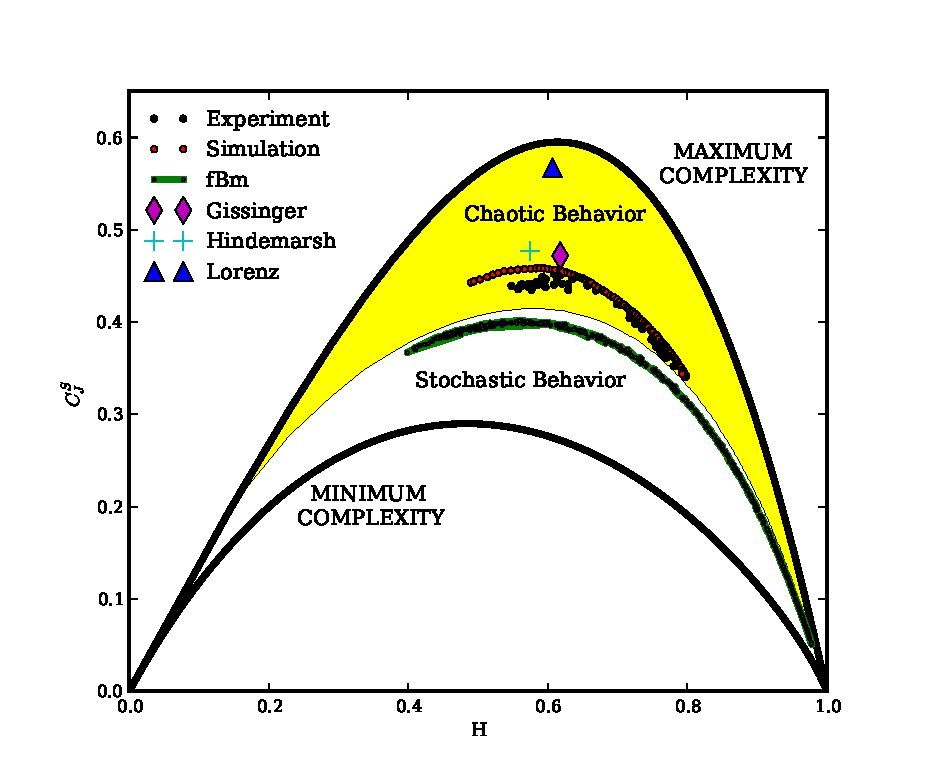
\includegraphics[]{entropy_complexity}}
\caption{Location of data in the entropy-complexity plane}
\label{entropy_complexity}
\end{figure}

The CH plane is actually bounded by two curves that define the minimum and maximum and the possible complexity as a function of entropy 
for a probability distribution with a given number of elements. The probability
distributions that define these curves are explained by Maggs and Morales~\cite{maggs2013}. Specifically, I use $7!=5040$ elements, meaning that I use an embedding dimension $d_e$ of $7$
in the attractor trajectory reconstructions.

In this figure, for reference, I show two low-dimensional chaotic models -- the aforementioned Lorenz model~\cite{lorenz1963} and the Gissinger model~\cite{gissinger2012}. 
Both models contain three degrees of freedom and have low-dimensional chaotic attractors. I use subsampling rates of $\tau=16$ for the Lorenz model and $\tau=200$ for the Gissinger model, corresponding
to the optimal values obtained by the method I described above. I note that using an embedding dimension of $7$ is not optimal for these models -- it is actually too high -- but there is no
loss of trajectory information by using too high of an embedding dimension. The only problem is the need for larger amounts of data. I use this embedding dimension so that I can keep more
attractor information for the LAPD data, even though it is still too low. And I do not have enough data for any of the models to use higher than $7$. Both of these chaotic models sit near the
location of highest possible complexity in the CH plane, which is typical for chaotic models~\cite{rosso2007}.

Additionally, I show a number of green data points labeled 'fBm,' which stands for fractional Brownian motion. Rosso et al. explain fractional Browning motion and how to obtain the time signals
that lead to these different data points by varying the Hurst exponent~\cite{rosso2007}. 
To get the points from the time signals, I compute their permutation entropies and complexities using the embedding dimension of $7$ with no subsampling,
which is suggested for stochastic processes~\cite{riedle2013}. The important point is that fractional Brownian motion is a stochastic process with higher complexity than most other stochastic
processes. The curve mapped out by the points, therefore, serves as a kind of delimiter of stochasticity, where anything below this curve is stochastic. Chaotic and stochastic processes
sit in different locations of the CH plane, so determining the location in the CH plane of experimental or simulation data is a way to quantify the stochasticity of those data.

In that regard, I plot the location of the experimental and simulation data in the CH plane in this same figure. The different points correspond to a few different radial locations in order
to see if the turbulence at different radii has different dynamics. Again, I use an embedding dimension of $7$ and subsampling rates of $12$ for the simulation and $40$ for the experiment,
in accord with the results of Fig.~\ref{pe_lapd}. The embedding dimension here is too low, but it is the best I can do given data size limitations. Clearly, the experiment and simulation
data points are located right along the fractional Brownian motion curve in the CH plane. This indicates that the LAPD turbulence is stochastic but not highly so. This confirms that the dimensionality
of the LAPD turbulent attractors is high, though it is not clear how using too low an embedding dimension affects this result. Anyhow, this analysis does not provide a quantitative estimate
of the turbulent attractor dimension.

\section{Using the Proper Orthogonal Decomposition}
\label{s_pod_chaos}

The permutation entropy uses only the time signal of the data because it's based upon time delay attractor reconstruction. This makes it nice to use for experimental data, which is generally
restricted to time series data. But in this dissertation, I have argued and showed that a well-validated simulation can open up new forms of analysis that are not open to experimental data,
providing enhanced understanding of underlying turbulent processes. The same is true regarding the question of determinism versus stochasticity.

The key in using simulation data is that it contains detailed spatial information in addition to temporal information. In the case of chaotic analysis with simulation data, 
one does not need to reconstruct the attractor orbit because it is given by the spatio-temporal output of the simulation. The primary difficulty in understanding the chaotic nature of the simulation, 
then, is finding the effective degrees of freedom in which the attractor is embedded among the large number of available degrees of freedom. In my simulation model that has four differential
equations for the four independent variables, the number of degrees of freedom is $4 \times N_r \times N_\theta \times N_z$, where $N_j$ corresponds to the number of grid points that I use in each
respective direction. In fact, using a finite number of grid points already reduces the number of degrees of freedom from infinity to a finite number. Gridding assumes that the turbulence
can be described without an infinite number of degrees of freedom in that very small structures below the grid resolution cannot exist due to diffusive and viscous forces. 

I can go further by hypothesizing that there are a limited number of ``modes'' that effectively determine the turbulence. 
In other words, there exists some manifold in the phase space on which the attractor lies that has dimension less than that of the entire phase space. This, after all, is the assumption behind
the time delay embedding that allows for a low embedding number. So with the spatio-temporal simulation data available, it should be possible to find the relevant modes that control the turbulence
and project the turbulence onto these modes. The POD procedure, which I introduced in Sec.~\ref{s_pod} is perfect for this task. The reason is that the POD provides the optimal basis for
reconstructing the turbulence from the fewest possible modes, as described by Eq.~\ref{pod_optimality}. The POD procedure can be considered a way of rotating the phase space axes so that
the attractor lies in a hyperplane that can be described with as few coordinates as possible.

The way to quantify the number of effective degrees of freedom of the turbulence through the POD is by looking at the POD singular values $\sigma_q$. Recall that $\sigma_q^2$ is the time-averaged
amount of energy contained in POD mode $q$. If the top $10$ POD modes, for example, contain $90\%$ of the energy, then the projection of the turbulence onto the $10$ mode POD reconstruction
is $0.9$. This follows from Eqs.~\ref{svd}-~\ref{pod_truncation}. Clearly, the singular values correlate to the importance of the modes. To normalize the singular values to the total energy
of the turbulence, I define

\beq
\label{pj_def}
p_q = \sigma_q^2/E
\eeq
where $\sum_q p_q = 1$. The $p_q$'s then form a probability distribution. 

I perform a POD on the turbulent data of the Periodic simulation, using $300$ time points in the quasi-steady state stage of the simulation. 
For the POD, I do not use any Fourier transforms like I did in Sec.~\ref{ss_pod_dynamics}. Obviously, that would be inappropriate for my aim here.
I plot the $p_q$'s in Fig.~\ref{pod_sigmas} a), showing only every third $p_q$. The fairly rapid exponential decay of the POD energy fractions proves that the turbulence can be relatively well constructed
using a limited number of modes. In Fig.~\ref{pod_sigmas} b), I plot $\sum_q=1^Y p_q$ as a function of $Y$. This indicates how much of the turbulent energy is reproduced by the rank-$Y$ POD
reconstruction. From this calculation, I determine that the top $58$ POD modes contain $90\%$ of the turbulent energy. One might crudely conclude that the turbulence is governed by something
on the order of $100$ effective degrees of freedom. This is not low-dimensional chaos.

\begin{figure}[!ht]
\centerline{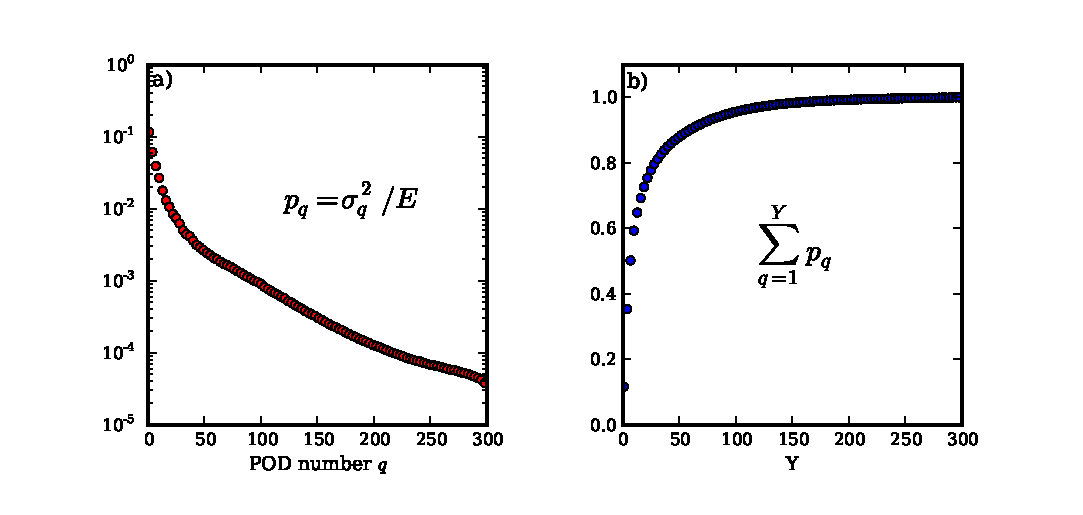
\includegraphics[]{pod_sigmas}}
\caption{Fractional energy content of POD modes}
\label{pod_sigmas}
\end{figure}

Now, an obvious practical problem with this is that every single POD mode contains at least some energy, so that one may never get a definitive answer on the number of effective degrees of freedom. 
Taking the number of modes that contain $90\%$ of the energy is quite arbitrary, as is using any other percentage. It would be convenient if the $p_q$'s became zero at some $q$, but this is not
the case, and it probabily never happens due to numerical noise of the POD procedure, which has been shown by Professor Paul Terry in unpublished work. The upshot
is that it is not possible to conclude exactly how many effective degrees of freedom there are based on the number of finite-energy POD modes. Probably, it is better to get a sense of how
deterministic or how stochastic a process is based on the rate of decline of the $p_q$'s. The results in the previous section suggest that the entropy and complexity are good ways
to test the stochasticity of a process, although rather than using permutation entropy, one uses the POD entropy. In fact, Futatani et al.~\cite{futatani2009} suggested the use of POD entropy as a way
to classify turbulence.

The normalized POD entropy, defined similarly to Eq.~\ref{perm_ent}, is

\beq
H_{{\rm{POD}}} = \sum_{q=1}^{N_{{\rm{POD}}}} p_q {\rm{log}}_2 (p_q)/ {\rm{log}}_2 (N_{{\rm{POD}}})
\eeq
and the complexity can be defined similarly following Eq.~\ref{csj}. The values that I obtain for the normalized POD entropy and complexity are $0.67$ and $0.35$, respectively. While this entropy
is about the same as what I found for the chaotic Lorenz and Gissinger models in the previous section, the complexity is much less. If I were to plot the POD entropy and complexity in the CH plane
of Fig.~\ref{entropy_complexity}, it would lie just below the fractional Brownian motion curve. It's not clear, however, how well the permuation entropy and complexity for a given embedding
dimension compare to the POD entropy and complexity. And, to further complicate matters, the POD entropy can be a function of the total number of POD modes used in the POD procedure, 
regardless of the normalization used in the entropy. To prove this, I define a POD entropy that is a function of the total number of POD modes ($T$) used to obtain the POD

\beq
H_{{\rm{POD}}}(T) = \sum_{q=1}^T p_q {\rm{log}}_2 (p_q)/ {\rm{log}}_2 (T).
\eeq
The proper way to find this, would be to perform the POD with a different number of time points, which would give a different number of POD modes. However, the POD takes a long time to calculate,
so this isn't feasible. Rather, by looking at Fig.~\ref{pod_sigmas} a), I reason that using more time points will simply extend the $p_q$'s along the exponential line. Using this logic, I create
series of $p_q$'s with different lengths and calculate the entropy as a function of the total length of the given series. In Fig.~\ref{pod_extended}, I plot the POD entropy $H_{{\rm{POD}}}$
as a function of the total mode number $T$ used in the POD. The blue curve that I call ``Constant Slope'' -- because I use a constant slope (in log space) to extend the series -- is this result.
Additionally, I plot the green curve in the same figure. For this curve, rather than extending the $p_q$'s with a constant logarithmic slope, I simply extend them to have the same value as the last
POD mode ($q=300$). I do this under the assumption that all POD modes beyond a certain point are simply due to noise of the POD calculation, so that they all contain the same energy.
These results indicate that the entropy is a function of the number of modes used in the POD; however, the entropies appear to level off at high $T$, suggesting that the actual
entropy may be the asymptotic value of $\sim 0.5$.

\begin{figure}[!ht]
\centerline{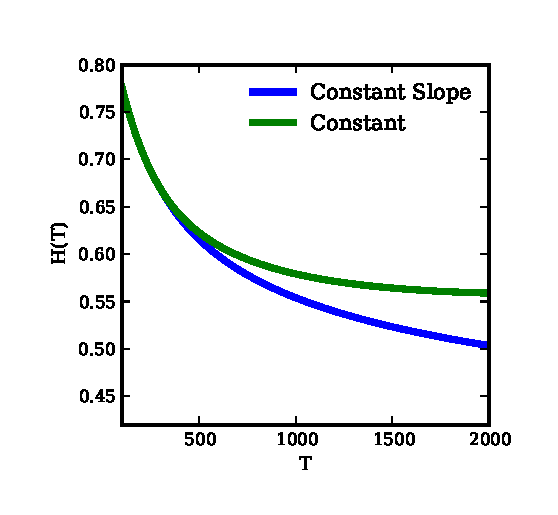
\includegraphics[]{pod_extended}}
\caption{POD entropy as a function of total mode number}
\label{pod_extended}
\end{figure}
